\documentclass{suturo}

\begin{document}
    \maketitle{Knowledge}{05.01.2018}{}{1}{}{}{}{}

\makeatletter
\newcommand{\chapterauthor}[1]{%
  {\parindent0pt\vspace*{-47pt}%
  \linespread{2.2}\large\begin{flushright}von: #1\end{flushright}%
  \par\nobreak\vspace*{0pt}}
  \@afterheading%
}
\makeatother

\section{Architektur und Funktion}
\subsection{kitchen\_model\_export}
\chapterauthor{Alexander Haar}
Das Kitchen\_Model\_Export-Paket dient dazu der Manipulation die Umgebung bekannt zu machen, damit der PR2 nicht mit der Umgebung kollidiert.

\begin{figure}[!htb]
        \center{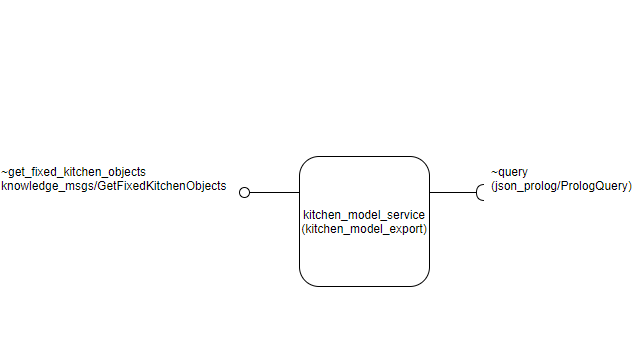
\includegraphics[width=\textwidth]
        {figures/kitchen_model_service.png}
        \caption{\label{fig:vision_node} Architektur der kitchen\_model\_service-node}}
\end{figure}
      
\section{API}
\subsection{kitchen\_model\_export}
\chapterauthor{Alexander Haar}

\subsubsection{prologValueToDouble}
\begin{verbatim}
double prologValueToDouble(PrologValue value)
@params: PrologValue welcher zu einem Double konvertiert werden soll
@return: Der aus der Konvertierung resultierende Double 

Description: Konvertiert ein PrologValue zu einem Double
\end{verbatim}\label{func:findcluster}

\subsubsection{prologBindingToQuaternion}
\begin{verbatim}
tf::Quaternion prologBindingToQuaternion(PrologBindings bdg)
@param: Die zu verarbeitenden PrologBindings(bdg["Quaternion"])
@return: Das aus den PrologBindings extrahierte Quaternion

Description: Extrahiert aus PrologBindings(bdg["Quaternion"]) das Quaternion und gibt es
als tf::Quaternion zurück
\end{verbatim}\label{func:findcentergazebo}


\subsubsection{prologBindingToPosition}
\begin{verbatim}
tf::Vector3 prologBindingToPosition(PrologBindings bdg)
@param: Die zu verarbeitenden PrologBindings(bdg["Translation"])
@return: Die aus den PrologBindings extrahierte Position

Description: Extrahiert aus PrologBindings(bdg["Translation"]) die Position und gibt es als tf::Vector3 zurück
\end{verbatim}\label{func:findcenter}

\subsubsection{toPoseMsgs}
\begin{verbatim}
geometry_msgs::Pose toPoseMsgs(PrologBindings bdg)
@param: Die zu verarbeitenden PrologBindings(bdg["Translation"] & bdg["Quaternion"])
@return: Die aus den PrologBindings extrahierte Pose

Description: Extrahiert aus PrologBindings(bdg["Translation"] & bdg["Quaternion"]) die Pose und gibt diese als geometry_msgs::Pose zurück
\end{verbatim}\label{func:estimatesurfacenormals}

\subsubsection{toBoundingBoxMsgs}
\begin{verbatim}
geometry_msgs::Vector3 toBoundingBoxMsgs(PrologBindings bdg)
@param: Die zu verarbeitenden PrologBindings(bdg["BoundingBox"])
@return Die aus den PrologBindings extrahierte BoundingBox

Description: Extrahiert aus PrologBindings(bdg["BoundingBox"]) die BoundingBox und gibt diese als geometry_msgs::Vector3 zurück
\end{verbatim}\label{func:createpointnormals}
\section*{Schnittstellen}
\chapterauthor{Alexander Haar}

\subsection*{Service Server kitchen\_model\_export/get\_fixed\_kitchen\_objects}
\begin{verbatim}
GetFixedKitchenObjects.srv
@request: -
@response: string frame_id
           string[] names
           geometry_msgs/Vector3[] bounding_boxes
           geometry_msgs/Pose[] poses
\end{verbatim}
Gibt im map- Frame alle Kollisionsobjekte für die Planning- Scene auf Anfrage zurück. Ein Kollisionsobjekt wird durch eine Box und eine Pose beschrieben, sowie einem Namen zur Identifizierung.

\section{Programmablauf}
\subsection{kitchen\_model\_export}
\begin{itemize}
\item[1.]Es wird eine Anfrage an den Service-Server gestellt
\item[2.]Eine Anfrage mit folgendem Inhalt wird an den json\_prolog- Server wird gestellt: "get\_fixed\_kitchen\_objects(ObjectName, Translation, Quaternion, BoundingBox)" 
\item[3.]Alle SemanticMapPerceptions aus der room.owl werden entsprechend ausgewertet und zurückgegeben.
\item[4.] Die als PrologBindings vom json\_prolog- Server erhaltenen werden mit den eigens in C++ implementierten Methoden in die gewünschte Form konvertiert
\item[5.] Antwort zurückgeben
\end{itemize}

\end{document}
